\documentclass[10pt,a4paper]{article}
\usepackage[utf8]{inputenc}

% \usepackage{ngerman}  % german documents
\usepackage{graphicx}  % import graphics einbinden
\usepackage{listings}  % support source code listing
\usepackage{amsmath}  % math stuff
\usepackage{amssymb} % 
\usepackage{a4wide} % wide pages
\usepackage{fancyhdr} % nice headers
\usepackage{float}
\usepackage{longtable}
\usepackage{xcolor}
\usepackage{cite}
\usepackage{fancyhdr}
\usepackage{tabularx}
\usepackage{booktabs}
\usepackage{lscape}
\usepackage{gensymb}
\usepackage{textgreek}

\usepackage[pdfpagemode=None, colorlinks=true,  % url coloring
linkcolor=blue, urlcolor=blue, citecolor=blue, plainpages=false, 
pdfpagelabels,unicode]{hyperref}

\definecolor{darkpastelgreen}{rgb}{0.01, 0.75, 0.24}
\definecolor{spirodiscoball}{rgb}{0.06, 0.75, 0.99}
\definecolor{smalt}{rgb}{0.0, 0.2, 0.6}
\definecolor{armygreen}{rgb}{0.29, 0.33, 0.13}
\definecolor{awesome}{rgb}{1.0, 0.13, 0.32}
\definecolor{bittersweet}{rgb}{1.0, 0.44, 0.37}
\definecolor{bananayellow}{rgb}{1.0, 0.88, 0.21}
\definecolor{blue}{rgb}{0.0, 0.0, 1.0}
\definecolor{red}{rgb}{1.0, 0.0, 0.0}
\definecolor{green}{rgb}{0.0, 1.0, 0.0}





\title{\Huge Bioinformatics Practicals In Sillico \\ \textbf{\normalsize BC-7107}}

%\raggedright
%
\includegraphics[width = 40mm]{img/unibe.png}\\[8ex]

\vfill
%set up names, matricle number, and email
\author{
	\noindent
	\begin{tabular}[t]{@{}l}
		\href{mailto:thibault.schowing@unifr.ch}{Thibault Schowing}\\
		\href{mailto:lio_roh@students.unibe.ch}{Lionel Rohner}\\
		\href{mailto:alain.rohrbasser.unifr.ch}{Alain Rohrbasser}\\
		\href{mailto:rares.cristea@unifr.ch}{Rares Cristea}
	\end{tabular}
		}

%\hfill
%\raisebox{\dimexpr.8\baselineskip-\height}{\includegraphics[width=32mm]{example-image}}


\begin{document}

\clearpage\maketitle
\thispagestyle{empty}
\newpage

\pagestyle{fancy}             % header
\setcounter{page}{1}

%lecture name
\newcommand{\lecture}{
	Bioinformatics Practicals In Sillico
}           

%assignment iteration
\newcommand{\assignment}{
	BC-7107
}


\setlength \headheight{25pt}
\fancyhead[R]{\begin{tabular}{r}\lecture \\ \assignment \end{tabular}}
\fancyhead[L]{HS-2019}

\part*{Introduction}

Bioinformatics is the application of computational technology to handle the rapidly growing repository of information related to molecular biology. Bioinformatics combines different fields of study, including computer sciences, molecular biology, biotechnology, statistics and engineering. It is particularly useful for managing and analysing large sets of data, such as those generated by the fields of genomics and proteomics.\\

In this report we focus on the bioinformatics tools for mutant analysis through three different projects; mutations in gai and spy in \textit{Arabidopsis Thaliana}, mutations in \textit{Saccharomyces cerevisiae} and mutations as well as Denovo assembly in \textit{Lactobacillus Helveticus}. We want to sort out new mutations with these tools and learn how to design a bioinformatic test. It includes the quality test, the annotation of our sequenced genomes and various analysis of these results. Thus, everything upstream of the analysis must be properly done, using several software described thereafter. Our machines are too week in order to analyse the data and performed the bioinformatics steps, thus, we will use a cluster dedicated for this lecture, in Bern Switzerland. 




\newpage
\part*{Yeast Genome Analysis}

\section*{Introduction}

%\paragraph{Biological introduction}The budding Yeast Saccharomyces cerevisiae is a common organism used for genetics manipulation. This organism is well conserved among the eukaryote and can be used correlate with human pathways. With a genome with 16 chromosomes (haploid, Mat a or $ \alpha $) or 32 chromosomes (diploid). 99\% of the genome is without introns, make this organism handy to manipulate. 12 million bases pair and contains between 5 800 to 6 572 genes %TODO ref. 

%The homology with human is estimate to 23\%, which is a good candidate for preliminary studies regarding human pathways. The short mating time and growth is also short. Thus, the identification of potential mutant is grandly enhanced. This is a single eukaryotic organism with a division cycle of 90 minutes. Through the process of budding in which smaller daughter cells pinch, or bud, off the mother cell. Due to the microscopic size ($~$5 microM, between bacteria and human cell size) and simple growth environment, yeasts are inexpensive and easy to grow in silico. Saccharomyces cerevisiae is also no-pathogen, and forms colonies on agar plates in the laboratory in a few days with no special incubators required (best grow at 30 $ \deg $). 

The budding yeast \textit{Saccharomyces cerevisiae} (\textit{S.cerevisiae}) is a single-celled lower eukaryote belonging to the kingdom of fungi. Ever since its discovery, \textit{S.cerevisae} has nourished human advancements in the field of fermented food products, alcoholic beverages (e.g. beer, which is the epony of \textit{S.cerevisae}) and the production of biofuel. In addition to the contribution industrial fermentation, \textit{S.cerevisiae} has become one of the most popular model organism for eukaryotic biology, due to its simple cellular architecture, cheap maintenance cost, fast growth, non-pathogenic nature (discussed in \cite{perez-torrado_opportunistic_2016}) , and homologies to human cells (e.g. ribosomes), which cannot be studied in prokaryotic model organism, such as \textit{E.coli} \cite{botstein_yeast_2011}. In particular, the genetic analysis of \textit{S.cerevisiae} has gained popularity in the scientific community since it was the first eukaryotic organism whose genome was fully sequenced. The haploid genome of \textit{S.cerevisiae} consists of 16 linear chromosomes containing 6604 genes encoded within approximately 12 megabase-pairs (Mbp)\cite{belda_saccharomyces_2019}. The fact that genome of \textit{S.cerevisiae} is quite small and almost completely void of intronic DNA, thus making it an ideal microorganism for the identification of mutations and single nucleotide polymorphisms.\\

\noindent Mating of two haploid yeast of opposite mating type (i.e. Mat a or $\alpha $) gives rise to diploid cells that possess 32 chromosomes. This is a single eukaryotic organism with a division cycle of 90 minutes. Through the process of budding in which smaller daughter cells pinch, or bud, off the mother cell. \textit{S.cerevisiae} forms colonies on agar plates in the laboratory in a few days with no special incubators required (best grows at 30\degree C).\\


%todo tom 1
\textbf{TODO raccourcir intro}

\paragraph{Target of Myb protein1 (Tom1)}, is a gene involved in the ribosomal biogenesis in yeast and human respectively. In human, this gene is involved in several pathways including endocytosis, endosomal transport, intracellular protein transport, neutrophil degranulation and protein transport\cite{seroussi_tom1genes_1999,seet_endofin_2004}. It is located on the ch.22 (component UP000005640) and ch.4 in human and yeast respectively. As it is well conserved among the eukaryote, we can study the gene with yeast for the raisons explained above. In yeast specifically, TOM1 was first described as a gene involved in temperature sensitivity and could be supressed by STM1\cite{utsugi_high_1995}. TOM1 is a hect-domain, which has been identified as a conserved feature of E3 ubiquitin ligases group. It regulates transcriptional activation through effectors ADA on coactivator proteins on the DNA. The action of TOM1 is to regulate through ubiquitination the temperature sensitivity\cite{saleh_tom1p_1998}. \\

\noindent A tom1-1 mutant has been isolated, and under electron microscopy and indirect immunofluorescence microscopy, it has been shown that the large nucleus contains duplicated DNA and short spindle, and structures fragmentations. This show that the disruption of the system, impacts the nuclear transport and the cell division in the G1 phase\cite{seet_endofin_2004,utsugi_yeast_1999}.\\ 


\noindent TOM1 encode for a large 380KDa proteins with a hect-domain at his C terminus (homologous to E6-AO C terminus). Site-directed mutagenesis of the conserved cysteine residue (tom1C3235A) in the hect-domain, supposed to be necessary for thioester-bond formation with ubiquitin, abolished the gene function. After a test with the over production of a myc-tagged ubiquitinRA, it shows that TOM1 is a ubiquitin ligase\cite{utsugi_yeast_1999}. More recently, TOM1 has been described as a fundamental macromolecular machine. The ribosomes biogenesis is much more complex in eukaryote cells as in bacteria, and it is involved in several fundamental cellular processes, including growth and cell division\cite{dinman_eukaryotic_2009}.\\

\noindent Ribosomes are subunits assemblages allowing the production of proteins. Subunits are made of RNA (rRNA) and specifies proteins (r-proteins) (\textit{Saccharomyces cerevisiae}: 40S [18S rRNA, 33 RPs]; 60S [25S, 5.8S, 5S rRNA, 46 RPs]– \textit{Escherichia coli}: 30S [16S rRNA, 21 RPs]; 50S [23S, 5S rRNA, 34 RPs])\cite{kressler_driving_2010}. Recent studies have shown that defect in the biogenesis linked to a wide range of hereditary diseases like Alzheimer’s and anemia\cite{makioka_immunolocalization_2016}. Ribosomes are a mixture of almost 80 different protein and stick together through a scaffold made by the RNA as explain above. Each protein is expressed in one copy and each of these proteins are needed to assemble the ribosomes. However, the number of steps needed for the biogenesis is large and not totally known. Moreover, it is impossible for a cell to produce the exact number of the needed proteins, including the same number of copies of all the proteins needed in a ribosome\cite{sung_conserved_2016}. It will build up an approximate number needed and then degrade the leftovers, that will be ubiquinined by TOM1 and degraded in lysosomes. We can say that TOM1 act as a quality control on this mechanism during the anabolism and division phases of the cells, leading to a week and crucial homeostasis\cite{sung_conserved_2016}.\\

\noindent Ribosome biogenesis is an intricate process involving many chaperons and assembly factors ($>$200 factors) and snoRNAs (75)\cite{kressler_driving_2010}. Two subunits are part of the final ribosomes, the 40S has one rRNA (18S) and 33 r-proteins. The 60S comprises three rRNAs (25S, 5.8S, 5S) and 47 r-proteins subunit\cite{kressler_driving_2010}.\\


\noindent The assembly and maturation of the ribosomes passes from the nucleus to the cytosol. ATP-dependent RNA helicases and three AAA-type ATPases (ATPases associated with various cellular activities) are mandatory nedded to make this process occure.This suggests that the energy derived by these enzymes is required for ribosomes assembly. The absence of one of these proteins might stall ribosome biogenesis and terminate cell growth even under optimal growth conditions\cite{dinman_eukaryotic_2009,kressler_driving_2010}.\\

\noindent To summarize, TOM1 is necessary to the ribosome’s biogenesis and the elimination of the leftover building blocks by ubiquitination. Thus, the aim of this project is to identify the suppressor of this gene by high sequencing throughput with bioinformatics tools. \\

\textbf{TODO on en fait référence nule part à cette figure -> nécessaire ?}
\begin{figure}[h]
	\centering
	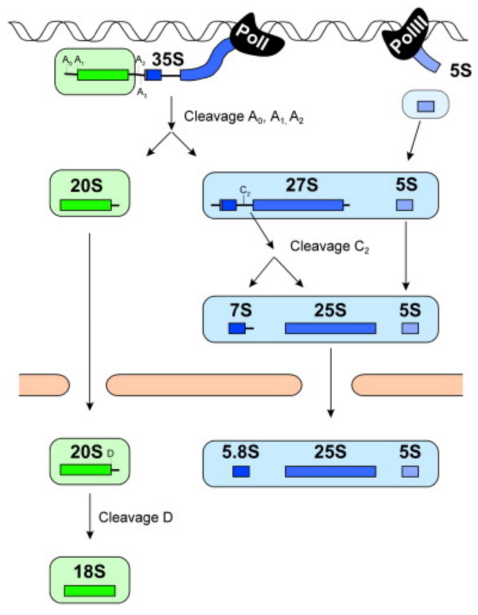
\includegraphics[width=0.4\linewidth]{img/tom1Intro}
	\caption{\small Simplified overview of the major steps in pre-rRNA processing.}
	\label{fig:tom1intro}
\end{figure}


%\paragraph{\textit{tom1}} The deletion of Tom1 has been associated with aggregation of ribosomal proteins, which results in a temperature-sensitive phenotype of S.cerevisiae that renders them incapable of growing at temperature exceeding 20\degree C. \\

%The aim of this study is to screen several $ \Delta $tom1 \textit{S.cerevisiae} strains for mutations in genes associated to tom1 (positive and negative regulators) and genes coding for riboproteins. \\

%In this project, we present a number of potential candidates that might help deciphering the temperature-sensitive phenotype of $ \Delta $tom1 \textit{S.cerevisiae}.


\section*{Methods}

\paragraph{Quality control of sequences} The high throughput sequencing method is not infallible, so the data will have contaminants, badly read sequences due to the intensity of the fluorescent signal, or the quality of the reagents that have a decaying quality with the number of sequencing cycles over time\cite{abnizova_computational_2017}. These errors might add a lot of false signals, useless extrawork, and complicate the data analysis, therefore we need to get rid of them. In order to check for the quality of the data, we use the tool : \textit{fastqc}\cite{andrews2012} which will help us visualize our fasta file given by the sequencer. \\


\paragraph{Trimming and bad quality reads removal } After the quality control check, we used the tool \textit{trimmomatic}\cite{bolger_trimmomatic:_2014} with the given parameters of MINLEN : 130 to trim down the bad quality ends of the reads, keeping at least 130bp of the trimmed read, and the parameter SLIDINGWINDOW:4:15, thus removing the reads that have an average base pair quality score lower than 15. The next step was checking if the quality of the data has improved after the trimming process, by using again fastqc, on the trimmomatic fastq file output.

\paragraph{Sequence alignment against reference} Since the fasta files gives no information about the sequences position in the yeast genome, we had to align all of the reads against the fasta file of a known yeast genome, or most likely a consensus of a yeast genome, containing the positional information.\\
 
\noindent However, in order to do that, we first had to index the reference fasta using the \textit{bwa index} tool\cite{li_fast_2010}, which is a way of giving a sort of table of contents of our reference fasta file (in our case the \href{https://www.ensembl.org/Saccharomyces_cerevisiae/Info/Index}{R64-1-1.92.fa}), that is used by the burrows-wheeler aligner algorithm. Subsequently, we used the \textit{bwa mem} tool in order to align our sequenced data against the reference. Then, we have converted all the SAM\cite{li_sequence_2009} files containing our aligned sequences, into BAM files, a compressed binary format easier to work with.
 
\paragraph{Variant calling and annotation}
This has been done using only \textit{samtools mpileup}, that took our reference file, and the aligned BAM files as an input, and gave us the binary format of the \textit{Variant Calling Format} files (.vcf). Then we used \textit{bcftools} to convert them into vcf.gz files. This method was prefered considering the fact that our genome is a haploid yeast genome, and it doesn’t need a complicated algorithm as used by the \textit{GATK} pipeline. The \textit{tabix}\cite{li_tabix:_2011} tool was used on the vcf files, in order to index them properly.\\

\noindent In order to annotate the variants given by the vcf files, we had to use \textit{SNPeff} tool on the vcf files that were merged together with all their indexes, and we also kept only the variants that were found in less than all 4 strains that we had to analyse, since we had to filter through all the variants that were different from the reference. The variants interesting to us, are indeed the ones that are specific to one of the mutants, and that’s why we had to filter this way.\\

\noindent The results were then visualized by either reading the vcf files in xcel or in IGV (\href{http://software.broadinstitute.org/software/igv/}{Integrative Genomics Viewer}).\\


%todo 
\textbf{TODO sources de l'image ?}

\section*{Results}
During our practical we screened the \textit{S.cerevisae} samples T5, T6, T7 and T8 for interesting mutations that could potentially be responsible for reverting the heat-sensitive phenotype of $\Delta$TOM1 \textit{S.cerevisae} strains. The sample T5 contains only one haploid strain named YDK1364 and was used as a reference (Figure \ref{fig:yeastgrowth}). All strains found in T6 to T8 arose from the strain YDK1364 found in T5, but as mutations emerged in strains S1364-1 to S1364-8, these strains became more resistant to high-temperature stress (i.e. 37\degree C). Therefore, we excluded all mutations that co-occurred in T5 and any of the samples of interest T6 to T8. Since each of the samples is composed of two pooled haploid \textit{S.cerevisae} strains (Figure \ref{fig:yeastgrowth}), we excluded all homozygous mutations from further analysis, since it is highly unlikely that two strains have the same mutation suppressing the $\Delta$TOM1 heat sensitivity phenotype.

\begin{figure}[h]
	\centering
	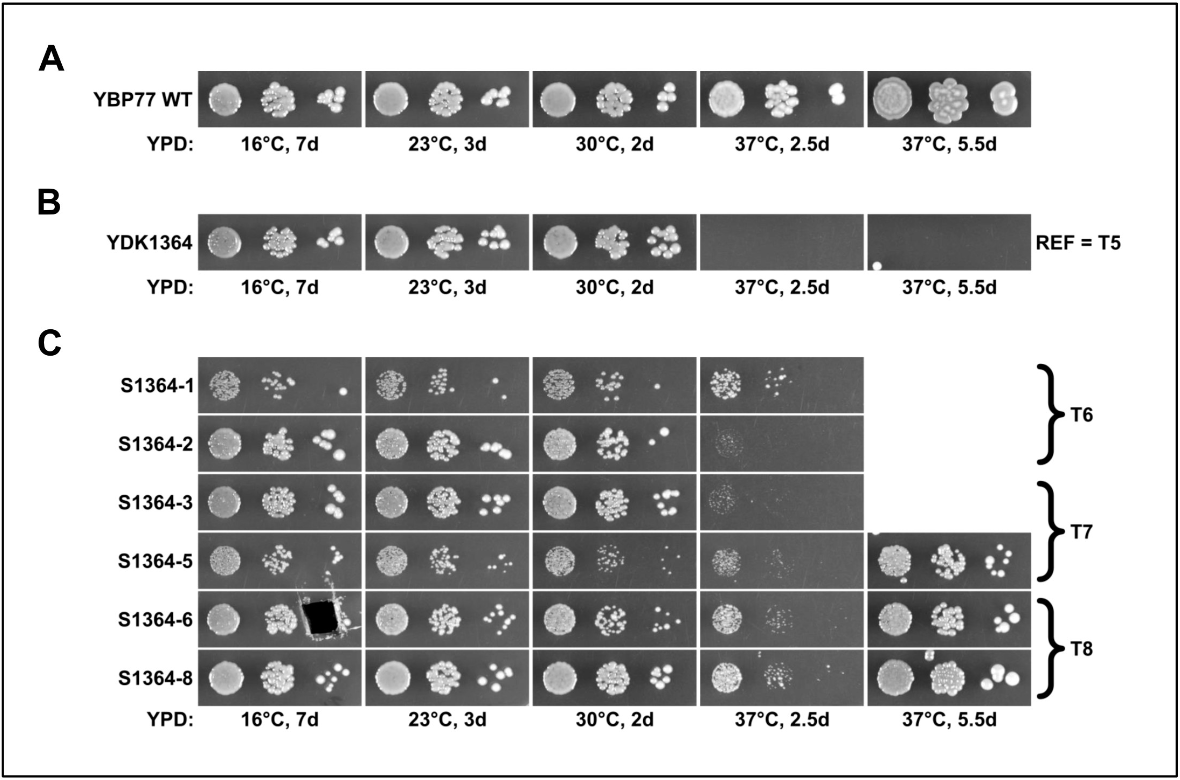
\includegraphics[width=0.7\linewidth]{img/yeastgrowth}
	\caption{\small Growth characteristics of \textit{S.cerevisae} strains cultured in Yeast Extract–Peptone–Dextrose medium (YPD) at different temperatures. Strain names are indicated on the left of the growth assay photographs. \textit{S.cerevisae} cells were plated onto agar plates and were cultured for up to 7 days at increasing temperature starting from 16\degree C to 37\degree C. (A) Wildtype yeast grows well at all tested temperatures. (B) Depicted is the growth behaviour of the $\Delta$Tom1 strain YDK1364, which is highly sensitive to heat. (C) Growth of mutated $\Delta$Tom1 yeast strains derived from YDK1364 that exhibit lower heat susceptibility due to accumulation of mutations that counteract the $\Delta$Tom1 phenotype. Depicted are representative growth assays of the different yeast strains. Adapted from course BC.7107, UNIFR, Benjamin Pillet.}
	\label{fig:yeastgrowth}
\end{figure}


\noindent In this first screening approach, we included only mutations with a Phred-scaled quality score of over 200. Furthermore, we focussed on mutations that interact genetically or physically with TOM1 or genes that encode for ribosomal proteins of the large (RPL) or small (RPS) subunit, because they have observed to accumulate and form detergent-insoluble. Using our pipeline described in the Variant calling and annotation of the Methods section, we identified nine mutations that may explain why samples T6, T7, and T8 are less susceptible to high temperatures compared to our reference T5.

% Please add the following required packages to your document preamble:
% \usepackage{graphicx}
% Please add the following required packages to your document preamble:
% \usepackage{booktabs}
% \usepackage{graphicx}
% Please add the following required packages to your document preamble:
% \usepackage{graphicx}
% Please add the following required packages to your document preamble:
% \usepackage{graphicx}
\begin{table}[]
	\tiny
	\centering
	\resizebox{\textwidth}{!}{%
		\begin{tabular}{|l|l|l|l|l|}
			\hline 
			\textbf{Sample} & \textbf{Gene Name} & \textbf{Mutation Type} & \textbf{Chromosome} & \textbf{Interactors} \\ \hline
			\textbf{T6} & YGR160W & \begin{tabular}[c]{@{}l@{}}Inframe\\ insertion\end{tabular} & VII & Unknown \\ \hline
			\textbf{T6} & PMT1 & Frameshift & IV & HAS1 \\ \hline
			\textbf{T7} & KRE6 & \begin{tabular}[c]{@{}l@{}}Stop \\ gained\end{tabular} & XVI & \begin{tabular}[c]{@{}l@{}}TOM1,\\   RPL1B, RPL34B\end{tabular} \\ \hline
			\textbf{T7} & KRE9 & Missense & X & \begin{tabular}[c]{@{}l@{}}MRPL17,\\   MRPL25, MRPL38,\\   RPL10, RPL11B,\\   RPL15A, RPL1B,\\   RPL24A, RPL2A,\\   RPL3\end{tabular} \\ \hline
			\textbf{T7} & ISC1 & Missense & V & RPL40B \\ \hline
			\textbf{T7} & FLO9 & \begin{tabular}[c]{@{}l@{}}Inframe \\ insertion\end{tabular} & I & IMG2, YAR1 \\ \hline
			\textbf{T7} & VTC4 & Missense & X & TOM1 (Physical) \\ \hline
			\textbf{T8} & KRE6 & Missense & XVI & \begin{tabular}[c]{@{}l@{}}TOM1, RPL1B, \\   RPL34B\end{tabular} \\ \hline
			\textbf{T8} & ROT1 & Missense & XIII & RPL4B, RPS25A \\ \hline
		\end{tabular}%
	}
\caption{\small Table depicting all heterozygous mutations found in the sample T6 to T8, which might be potential suppressors of the $\Delta$TOM1 phenotype.  Annotation of the mutation type was done by SnpEff. With the exception of VTC4, only genetic interactions are shown. All intergenic and synonymous mutations were excluded from further analysis.}
\label{tab:mutationT68}	
\end{table}

\section*{Discussion}

In sample T6, we found two potential high-quality mutation candidates, namely an inframe insertion in YGR160W and frameshift mutation in PMT1. On closer inspection, we found that YGR160W was flagged as a dubious gene, which is unlikely to encode a functional protein, thus in spite of the quality we discarded it from further research. In contrast, PMT1 codes for an O-mannosyltransferase that is involved in ER quality control among other things\cite{strahl_pmti_1993}\cite{goder_protein_2011}.\\

\noindent As a result of the enormous global genetic interaction network that has been created by M. Constanzo and colleagues, PMT1 has been shown to genetically interact with HAS1, which codes for an ATP-dependent RNA helicase that is involved in the biogenesis of the 40S and 60S ribosome subunits\cite{costanzo_global_2016} \cite{dembowski_has1_2013}.\\ 

\noindent In sample T7, we found an already described $\Delta$TOM1 suppressor gene named KRE6 as well as some putative candidates that might be worth investigating in more depth. In T7, we identified a nonsense mutation in the known extragenic suppressor KRE6 of $\Delta$Tom1. The premature stop codon is inserted at nucleotide position 1431 of 2161, which strongly suggests that translation of the KRE6 transcript results in the formation of a truncated protein. KRE6 codes for a type II membrane protein involved in the synthesis of $\beta$-(1,6)-glucan, which is an essential constituent of the fungal cell wall\cite{kurita_kre6_2011, roemer_skn1_1993}.\\

\noindent In spite of the fact that the function of the KRE6 protein is not directly involved stress responses, Sasaki and colleagues found that mutation in the KRE6 gene acts as a weak suppressor of heat sensitivity mediated by TOM1 deletion\cite{sasaki_extragenic_2000}.\\

\noindent Although the authors were not able to decipher the underlying mechanism responsible for restoring heat tolerance in $\Delta$TOM1 S.cerevisae with mutated KRE6, but they concluded that the mutation may activate unknown suppressor genes of $\Delta$TOM1. According to the Biological General Repository for Interaction Datasets \href{https://thebiogrid.org/}{BioGRID}, KRE6 has been shown to exhibit genetic interaction with TOM1 itself as well as multiple genes coding for mitochondrial and cytoplasmic ribosomal proteins of the large subunit (Table \ref{tab:mutationT68}). Moreover, we found a missense mutation in gene KRE9, which is also involved to be involved in the synthesis of $\beta$-(1,6)-glucan like KRE6 protein. The deletion of KRE9  has long been known to have a deleterious effect on the growth of S.cerevisae by altering the composition of its cell wall and thus causes defects to its integrity\cite{brown_yeast_1993}.\\

\noindent Similar to KRE6, KRE9 also interacts with several gene coding for the small and large subunit of ribosomes (Table \ref{tab:mutationT68}). It is also conceivable that KRE9 mutation alone or in combination with the mutation in Kre6 has an impact on the transcription of ribosomal genes and thus may passively counteract the stress response associated with the accumulation of protein related to $\Delta$Tom1. Another gene related to ribosome biogenesis was also found to be mutated in sample T7, namely ISC1, which has been reported to interact genetically with RBL40B\cite{hoppins_mitochondrial-focused_2011}. While the protein ISC1 is not directly linked to the regulation of ribosome biosynthesis, RPL40B is involved in the maturation of the 60S ribosomal subunit\cite{fernandez-pevida_yeast_2012}. Interestingly, the null mutation of ISC1 has been associated with heat sensitivity, which implies that the mutation observed in sample T7 does not yield a non-functional protein. Therefore, we concluded that the mutation in ISC1 is most likely not responsible for counteracting the heat-sensitive phenotype resulting form the deletion of TOM1.\\

\noindent Last but not least, we also identified a mutation in a direct physical interactor of the TOM1 protein in sample T7 named VTC4, which is a component of the vacuolar transporter chaperone (VTC) complex\cite{muller_role_2003}. Unfortunately, the nature of the interaction between VTC4 and TOM1 is not described and thus it is not possible to evaluate whether a mutation in this gene has an impact on the $\Delta$TOM1 phenotype. A possible interesting scenario could be that TOM1 is an inhibitor of VTC4.\\
 
\noindent In T8, we observed a missense mutation in KRE6. In addition, we discovered another missense mutation in a gene named ROT1, which codes for a chaperone involved in protein folding\cite{takeuchi_saccharomyces_2008}. Similar to the other gene candidates, ROT1 also interacts genetically with ribosomal genes, namely RPL4B and RPS25A.\\
 
\noindent Interestingly, most of the mutations we found in samples T6, T7, and T8 were indirectly linked to ribosomal genes. These findings are of particular interest since deletion of TOM1 \textit{S.cerevisae} has been associated with greatly increased levels of ribosomal proteins. Under normal conditions, the E3 ubiquitin ligase TOM1 rapidly removes excess of ribosomal proteins via proteasomal degradation\cite{sung_conserved_2016}.\\
 

\noindent In conclusion, we found one known as well as seven potential new suppressors of $\Delta$TOM1. The known suppressor KRE6, has been found to be mutated in T7 and T8. Due to the heterozygosity of the mutation, we conclude that KRE6 may explain the partially restored capability of \textit{S.cerevisae} to grow at 37\degree C in one of the two strains found in each sample. However, it is important to note that while the mutation in T7 introduces a additional stop codon, the spontaneous mutation in T8 only affected one amino acid and consequently affects the function of the protein to a lesser extent (Table\ref{tab:mutationT68})\cite{sasaki_extragenic_2000}. Since most of the mutated genes found in our samples were associated with biogenesis or regulation of ribosomes, it would be interesting to investigate whether these mutations suppress the accumulation of ribosomal proteins in the absence of TOM1. Take together our data provide the basis for further investigations aimed at clarifying whether accumulation of ribosomal proteins may be causative of the heat sensitivity of yeast lacking TOM1.
 
 
 
 
 
 









%%%%%%%%%%%%%%%%%%%%%%%%%%%%%%%%%%%%%%%%%%%%%%%%%%%%%%%%%%%%
%%%%%%%%%%%%%%%%%%%%%%%%%%%%%%%%%%%%%%%%%%%%%%%%%%%%%%%%%%%%
%%%%%%%%%%%%%%%%%%%%%%%%%%%%%%%%%%%%%%%%%%%%%%%%%%%%%%%%%%%%
\newpage
\part*{Arabidopsis Thaliana Genome Analysis}

\textbf{TODO ALAIN: raccourcir}\\

\noindent\textbf{TODO LIONEL: CHANGER IMAGE}

\section*{Introduction}
The plant Arabidopsis thaliana is a genetic model worldwide used in plant biology since 1995, when it has been promoted as model for molecular genetics. The genome is entirely sequenced in 200. ATH is a diploid organism of 114,5 to 125 million base pairs within 5 chromosomes (haploid). The germination to mature seed is done about 6 weeks and easy to cultivate in restricted space and produce a lot of seed. A wide range of mutants are already available and it growth from year to another through multinational research community of academic, government and industry laboratories. The importance of ATH is crucial and invaluable resources to fight the loss of crops due to plants diseases.


%
%
%


\paragraph{GAI} 

Gibberellic-Acid Insensitive (GAI) is a gene in Arabidopsis thaliana in chromosome 1 
which is involved in the regulation of plant growth.  Precisely, it mediated the input 
signals and module the growth by decreasing the responsiveness to gibberellin\cite{peng_arabidopsis_1997}.
%http://genesdev.cshlp.org/content/11/23/3194.short
Gibberellin is a tetracyclic diterpenoid growth factor and influence essentially the stem 
elongation and other plant developmental processes\cite{hooley_gibberellins:_nodate}.
%https://link.springer.com/article/10.1007%2FBF00016489
The main mutation involved a deletion of a 17 amino acid segment. The gai allele contains
a deletion of 51-bp from within the GAI ORF ,from close to the N terminus and confers a 
dominant dwarf phenotype. The GAI (gai1-1 and gai 1-2, two mutations on the same gene)
protein as normally a length of 533 AA and is normally located in the nucleus. The deleted segment is shown in yellow for DELLA,
the common one\cite{peng_arabidopsis_1997,lee_gibberellin_2002}.
%doi:10.1101/gad.11.23.3194
%http://genesdev.cshlp.org/content/16/5/646
If it is mutated (gai) and the plant growth better, it is a gain of function gene, in contrary it is a loss of function. \\

The mutation in SPY (spy) is a suppressor of gai, conferring to the plant a normal phenotype. 
GA-deficient Arabidopsis mutants display characteristic phenotypes, including dark green leaves 
and a dwarf growth habit attributable to reduced stem elongation\cite{peng_arabidopsis_1997}.
%http://genesdev.cshlp.org/content/11/23/3194.short
The gai mutation affects GA reception or subsequent signal transduction and does not result in GA deficiency\cite{hooley_gibberellins:_nodate}.
%https://link.springer.com/article/10.1007%2FBF00016489


%\begin{figure}[H]
%	\centering
%	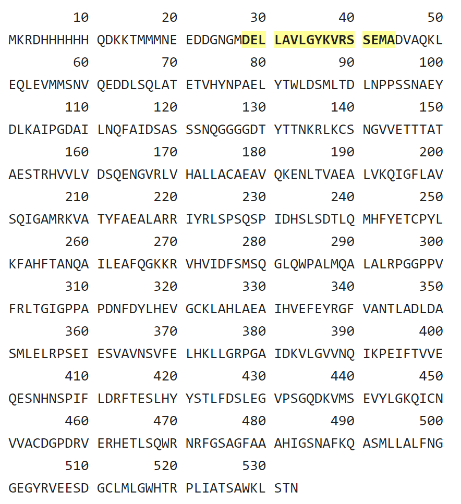
\includegraphics[width=0.4\linewidth]{img/dellamutation}
%	\caption{The DELLA protein GAI comes from the GRAS family protein 3 and located on the chromosome 1, locus:2006747 AT1G14920. Call DELLA because of the 17 AA deleted.}
%	\label{fig:dellamutation}
%\end{figure}





\paragraph{SPY}
For spy, three independent recessive mutations at the SPINDLY (SPY) locus of Arabidopsis confer resistance to the gibberellin (GA) biosynthesis inhibitor paclobutrazol. Paclobutrazol is a plant growth retardant. It is an antagonist of the plant hormone gibberellin. It works by inhibiting gibberellin biosynthesis by inhibiting endoplasmic reticulum monooxygenases. Relative to wild type, spy mutants exhibit longer hypocotyls, leaves that are a lighter green colour, increased stem elongation, early flowering, parthenocarpy, and partial male sterility. All of these phenotypes are also observed when wild-type Arabidopsis plants are repeatedly treated with gibberellin A3 (GA3). The spy-1 allele is partially epistatic to the ga1-2 mutation, which causes GA deficiency. In addition, the spy-1 mutation can simultaneously suppress the effects of the ga1-2 mutation and paclobutrazol treatment, which inhibit different steps in the GA biosynthesis pathway. This observation suggests that spy-1 activates a basal level of GA signal transduction that is independent of GA\cite{lee_gibberellin_2002}.
%http://genesdev.cshlp.org/content/16/5/646


%TODO remplacer par figure à Lionel
% \label{fig:gaspypathway}

\begin{figure}[H]
	\centering
	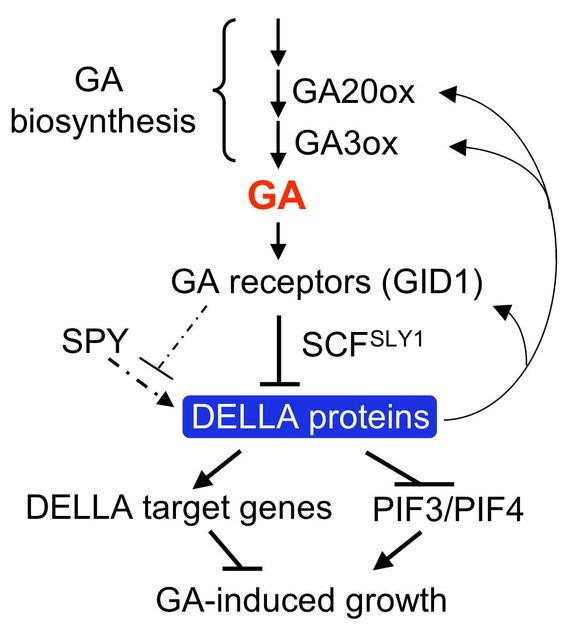
\includegraphics[width=0.4\linewidth]{img/GASPYpathway}
	\caption[GAI and SPY pathways]{https://www.ncbi.nlm.nih.gov/pmc/articles/PMC3243332/figure/i1543-8120-64-1-1-f21/}
	\label{fig:gaspypathway}
\end{figure}


\section*{Methods} 

\paragraph{Trimming, Read Group Informations, Aligning and MarkDuplicates} After the quality control check with \textit{fastqc}\cite{andrews2012}, \textit{Trimmomatic}\cite{bolger_trimmomatic:_2014} was used to filter out bad quality reads. Only the ones with a minimal length of 140 and an average quality of 15 were kept. The \textit{bwa} (Burrows-Wheeler Aligner) tool was then used to index the reference genome
%todo name and link to ref genome
and to align all the reads against this reference while adding the Read Group Information at the same time. The resulting sam files were then sorted and converted into bam files through  \href{https://software.broadinstitute.org/gatk/documentation/tooldocs/4.0.8.0/picard_sam_SortSam.php}{SortSam} (\href{https://broadinstitute.github.io/picard/}{Picard}) and the duplicate reads were marked using  \href{https://software.broadinstitute.org/gatk/documentation/tooldocs/4.0.4.0/picard_sam_markduplicates_MarkDuplicates.php}{MarkDuplicates} (\href{https://broadinstitute.github.io/picard/}{Picard}). This step, takes a sorted bam file and  add information about reads that might come from the same DNA fragment, in order to avoid counting the information given by one fragment more than one time. 

\paragraph{Haplotype Caller and Base Quality Score Recalibration} Since the genome of the \textit{Arabidopsis thaliana} is diploid, in order to analyse its sequences we had to use the \href{https://software.broadinstitute.org/gatk/documentation/tooldocs/3.8-0/org_broadinstitute_gatk_tools_walkers_haplotypecaller_HaplotypeCaller.php}{Haplotype Caller} (\href{https://software.broadinstitute.org/gatk/}{GATK4}), in order to have a first variant call. The vcf file was then split in two, one containing only the indel information, and one containing the SNPs, with  \href{https://software.broadinstitute.org/gatk/documentation/tooldocs/3.8-0/org_broadinstitute_gatk_tools_walkers_variantutils_SelectVariants.php}{SelectVariants} (\href{https://software.broadinstitute.org/gatk/}{GATK4}) because the filtration methods differ.Then the new vcf files were filtered to get rid of all the false variants, through  \href{https://software.broadinstitute.org/gatk/documentation/tooldocs/3.8-0/org_broadinstitute_gatk_tools_walkers_filters_VariantFiltration.php}{VariantFiltration} (\href{https://software.broadinstitute.org/gatk/}{GATK4}), using different parameters for indels and for SNPs.

% BQSR
% https://gatkforums.broadinstitute.org/gatk/discussion/44/base-quality-score-recalibration-bqsr  




\section*{Results} \textbf{TODO Rares}

\paragraph{Discussion}









%%%%%%%%%%%%%%%%%%%%%%%%%%%%%%%%%%%%%%%%%%%%%%%%%%%%%%%%%
%%%%%%%%%%%%%%%%%%%%%%%%%%%%%%%%%%%%%%%%%%%%%%%%%%%%%%%%%
\newpage
\part*{Lactobacillus Heleveticus Genome Assembly}
\section*{Introduction}

%todo core genome or pan-genome ?

The diverse bacteria involved in cheese production are essential for the texture and taste development but also, during the ripening process, the microbial changes helps to kill pathogens and reduce spoilage micro-organisms. \textit{Lactobacillus helveticus} is a thermophilic lactic acid bacterium (LAB) used in the dairy industry as a starter or an adjunct culture for cheese manufacture. By releasing \textbf{peptidoglycan hydrolases}(PGHs), it has the ability to digest the bacterial cell wall (gram+) inducing death of surrounding bacteria but also its own autolysis. \\

\noindent The genomic plasticity of \textit{Lactobacillus helveticus} leads to a high variation in PGHs activity from one strain to another. 
In a previous study\cite{jebava_nine_2011}, nine genes coding PGHs were annotated and the activity of a PGH with an estimated size of 30kDa was tested by zymography in nine strains of \textit{Lactobacillus helveticus} of which six were sequenced (see figure \ref{fig:zymography}). Two phenotypes were shown: phenotype A exhibits PGH activity (strains \textbf{FAM8102c1c1}, \textbf{FAM23285} and \textbf{FAM19191}) and phenotype B does not (strains \textbf{FAM22016}, \textbf{FAM1450} and \textbf{FAM1213}).\\

\noindent The aim of this work was to detect potential genomic differences involved in the two different phenotypes by sequencing, assembling and compare the genome of the six strains using a previously annotated reference genome of \textit{Lactobacillus helveticus} (\href{https://www.ncbi.nlm.nih.gov/genome/?term=NC_010080}{NC\_010080}). A potential candidate present only in the strains expressing a PGHs activity suggests that it might have been acquired by a viral insertion. 

  
%TODOOOOOOOOOOOOOOO

% BLASTP the protein sequence to see it comes from a phage !

\section*{Methods}

%TODO cite SOAPdenovo, Spades and Abyss
\paragraph{Sequencing and genome assembly}
The six \textit{Lactobacillus helveticus} strains \textbf{FAM8102c1c1}, \textbf{FAM23285}, \textbf{FAM19191}, \textbf{FAM22076}, \textbf{FAM1450}, \textbf{FAM1213}  were sequenced by Illumina sequencing. The following tasks were performed using the cluster provided by the University of Bern.  \textit{FastQC}\cite{andrews2012} was used to check the quality of the reads and \textit{Trimmomatic}\cite{bolger_trimmomatic:_2014} to filter out bad quality reads. Only the ones with a minimal length of 100 and an average quality of 8 were kept. \textit{SOAPdenovo} as well as \textit{Spades} were used to perform the genome assembly with the reads of each strains. For \textit{SOAPdenovo} the k-mer sizes were set to 95, 85, 75 and 65. For \textit{Spades} k-mere sizes were set to 21, 33, 55, 77 and 99 (default values). The four assemblies of SOAPdenovo and the assembly of Spades were compared using Abyss with a maximum number of contigs set to 1000. The best genome assemblies with the bigger N50 and a approximate genome size of 20Mbp (Genome size of \textit{Lactobacillus helveticus}) were then chosen\footnote{Due to the temporary unavailability of the cluster, this operation has been performed by L. Falquet and the results were provided to the students afterwards.}.


\paragraph{Genome annotation and pan-genome analysis}
We used the \textit{PROKKA} pipeline\cite{seemann_prokka:_2014} to annotate the genome of the six best assemblies and the reference genome for \textit{Lactobacillus helveticus} \href{https://www.ncbi.nlm.nih.gov/genome/?term=NC_010080}{NC\_010080}. \textit{PROKKA} is an automated pipeline that annotates prokaryotic genomes. It locates open reading frames ans RNA regions on contigs and translates it to protein sequences, searching for protein homologues in public databases. The resulting standards \href{https://www.ensembl.org/info/website/upload/gff.html}{.gff} files containing the annotated genome for each strain are then used by \textit{Roary}\cite{page_roary:_2015} to generate a pan-genome of the six strains. The result was then visualized with \textit{Phandango}\cite{hadfield_phandango:_2018} allowing visualisation of phylogenetic tree, associated metadata and genomic information.


\paragraph{Extraction of the genes for each phenotypes} Grep was applied to the files generated by \textit{Roary} to extract the nine PHG's \cite{jebava_nine_2011} labelled "Lhv\_" with \textit{PROKKA} (table \ref{tab:resultCommonLhv}). The set of genes found in strains expressing phenotype A was then compared to the set of gene showing phenotype B. In table \ref{tab:resultPGHexpr} we have the two PGHs present only in the three strains expressing the PGHs activity.  
%TODOAAAAAAAAAAAAAAAAAAAAa


\begin{figure}
	\centering
	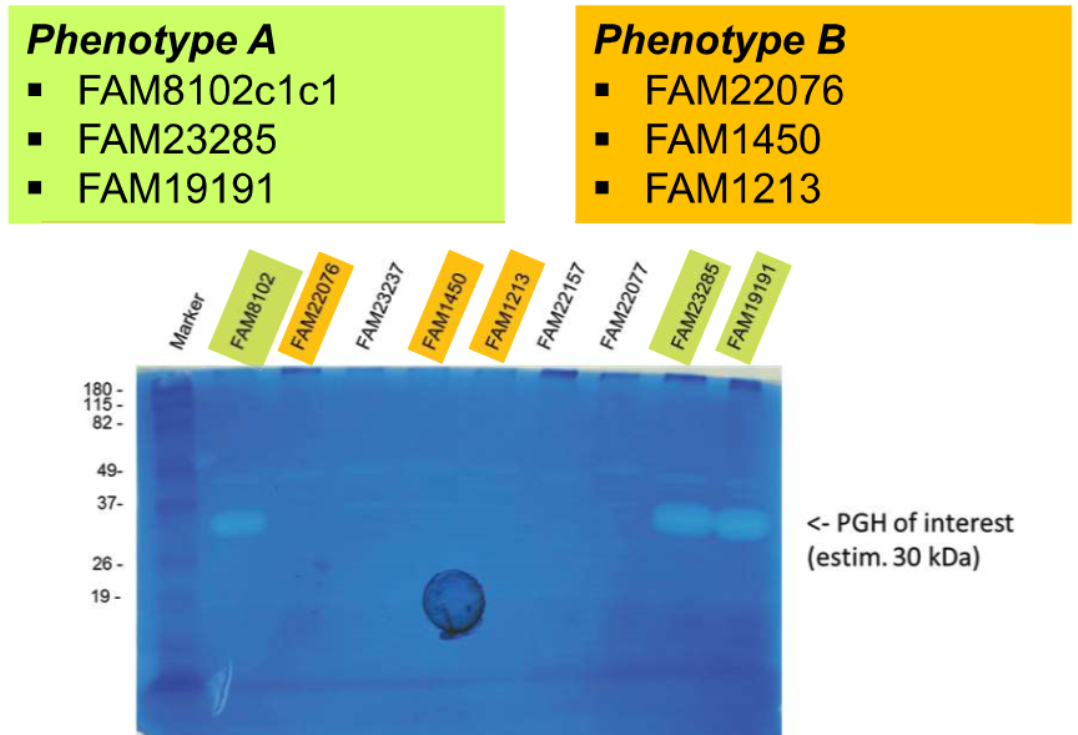
\includegraphics[width=0.7\linewidth]{img/zymography}
	\caption[The two phenotypes expressed by the six strains]{Phenotype A is expressing an active peptidoglycan hydrolase and phenotype B is not.}
	\label{fig:zymography}
\end{figure}


\section*{Results}



%TODO fix images


\begin{table}[htbp]
	\centering
	\begin{tabularx}{\linewidth}{|X|X|X|X|X|X|}
		\hline
		\textbf{Gene} & \textbf{Annotation} & \textbf{Avg group size nuc} & \textbf{FAM19191\_ 1K} & \textbf{FAM23285\_ 1K} & \textbf{FAM8102\_ 1K}\\
		 \hline
		%group\_1899 & Lhv\_2053 Lysin (L.crispatus) pseudogene in L.helveticus & 830/ 30 kDa & FAM19191\_ 1K\_00615 & FAM23285\_ 1K\_00607 & FAM8102\_ 1K\_00746 \\
		%\hline
		group\_2348 & Lhv\_2053 Lysin (L.crispatus) pseudogene in L.helveticus & 1121/ 41 kDa & FAM19191\_ 1K\_00069 & FAM23285\_ 1K\_00060 & FAM8102\_ 1K\_00069 \\
		\hline
		group\_2372 & Lhv\_2053 Lysin (L.crispatus) pseudogene in L.helveticus & 893/ 33 kDa & FAM19191\_ 1K\_00397 & FAM23285\_ 1K\_00499 & FAM8102\_ 1K\_00565 \\
		\hline	
	\end{tabularx}
	\caption{Genes present only in the three strains with a PGH activity.}
	\label{tab:resultPGHexpr}
\end{table}

\noindent According to figure \ref{fig:zymography}, the PGH involved is approximately 30kDa thus matches with group 2372. Looking at the alignment of the amino acid sequences (Figure \ref{fig:alignmentgrp2372}) we see that the sequences are identical thus showing a great conservation between the three strains. \\




\begin{figure}
	\centering
	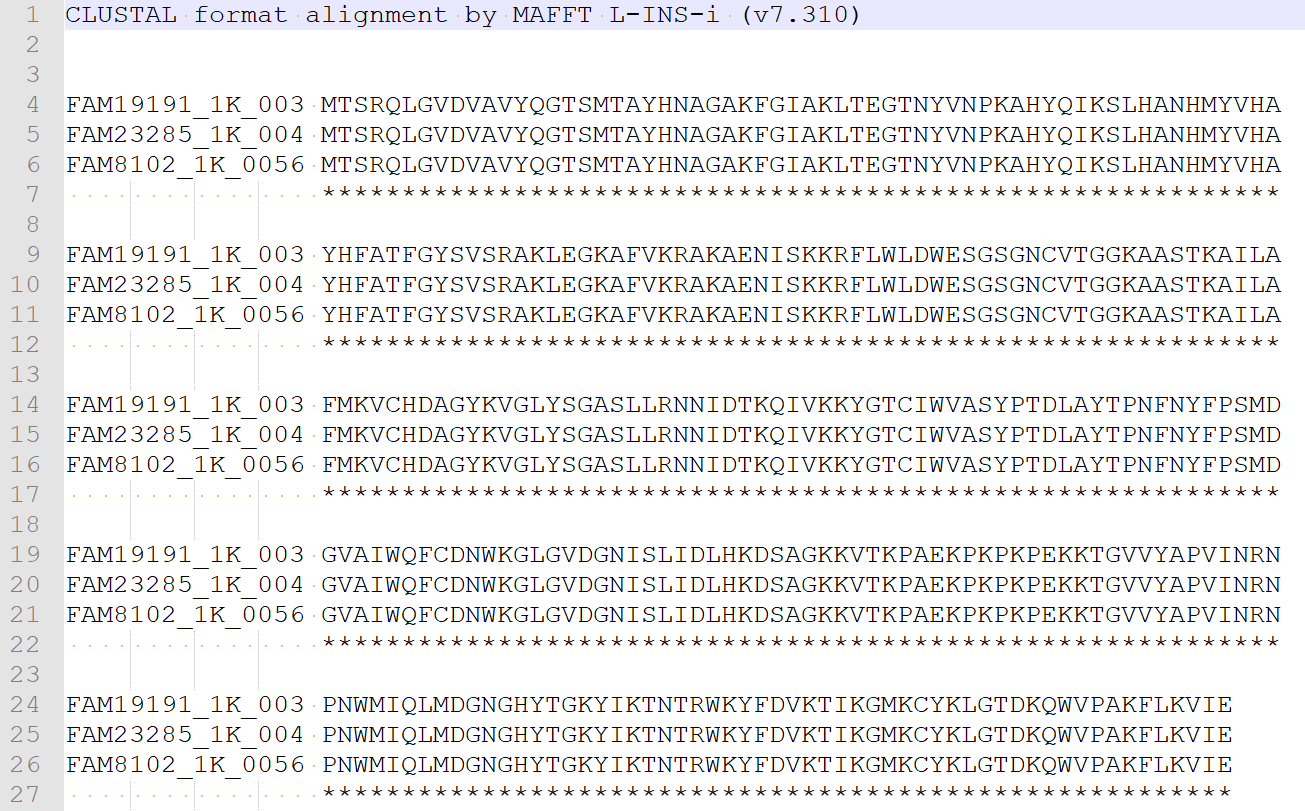
\includegraphics[width=0.7\linewidth]{img/AlignmentGrp2372}
	\caption{Alignment of amino acid sequences of group 2372 for the three strains.}
	\label{fig:alignmentgrp2372}
\end{figure}



%TODO align with mauve to reference (see script... fuck it)

%TODO check this paper : https://www.ncbi.nlm.nih.gov/pmc/articles/PMC6606699/ 




%todo discuss the results
\paragraph{Discussion} We can see that PGHs are present in all strains (Supplementary table \ref{tab:resultCommonLhv}), therefore the phenotype observed in the figure \ref{fig:zymography} is not due to an absence of PGH. With ROARY we identified a PGH only present in the three strains exhibiting phenotype A with a matching molecular weight.\\

\noindent Using BLASTp\cite{altschul_gapped_1997} with default parameters, the protein was searched to be a particular lysin (\href{https://www.ncbi.nlm.nih.gov/protein/1325986555}{WP\_101853908.1}) encoded by the pneumococcal bacteriophage Cp-1\cite{martin_pneumococcal_1998}. To look further into this sequence, we tried PHASTER \cite{arndt_phaster:_2016}, the PHAge Search Tool - Enhanced Release, which helps identifying and annotate prophage sequences within bacterial genomes and plasmids. The research was made only for \textbf{FAM19191}, as the sequence is identical in the three strains. The result indicating a highly conserved muramidase sequence, shown in figure \ref{fig:phasterresultmuramidase}, confirms that the PGH comes from a phage. The locus is shown in supplementary figure \ref{fig:circulargenomenode8annotated}.

\begin{figure}[H]
	\centering
	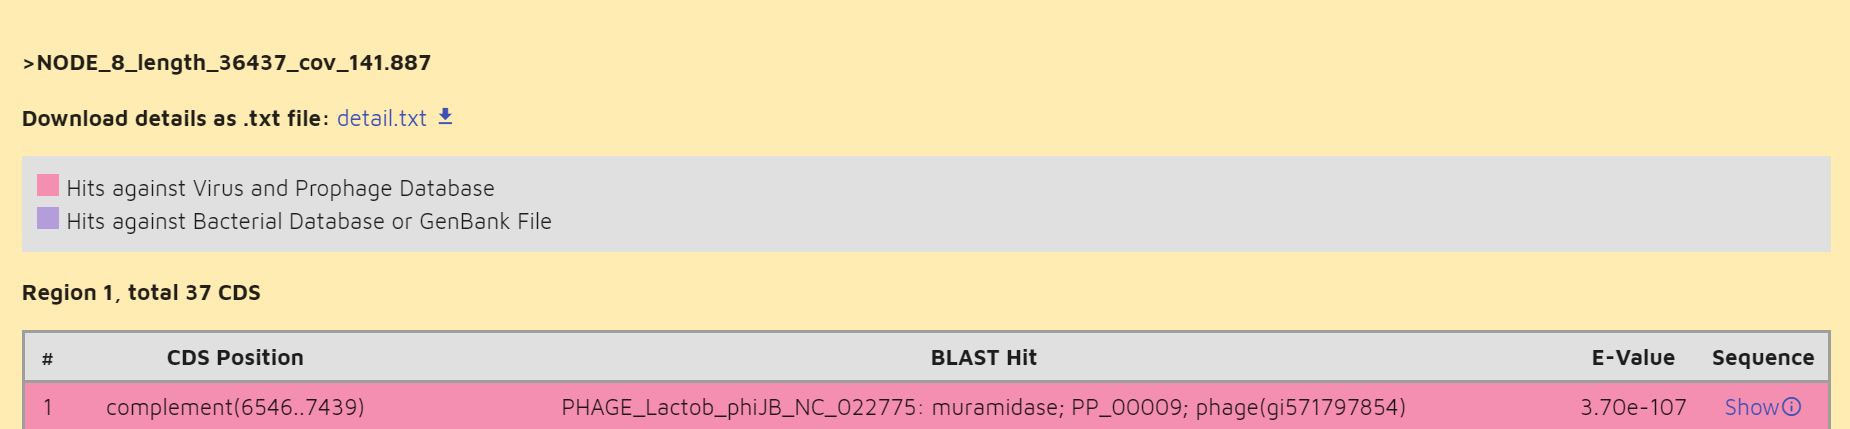
\includegraphics[width=1\linewidth]{img/phaster_result_muramidase}
	\caption{Partial result with the assembly of \textbf{FAM19191} run in PHASTER}
	\label{fig:phasterresultmuramidase}
\end{figure}

\noindent Many other genes sequences of other PGHs, pseudogenes or hypothetical proteins were found in some or all of the six different strains. It would be interesting to pursue further analysis of the transcription and expression of these sequences, to assess more precisely the differences between the strains.  

\newpage
\bibliography{mybib}{}
\bibliographystyle{ieeetr}

\newpage
\appendix
\part{Appendix}
\section{Supplementary figures Yeast Genome Analysis}


\section{Supplementary figures Arabidopsis Thaliana Genome Analysis}


\section{Supplementary figures Lactobacillus Helveticus Genome Assembly}

\begin{landscape}
	\begin{table}[]
		\begin{tabularx}{\linewidth}{|l|l|X|X|X|X|X|X|}\hline
			Gene & Annotation & FAM1213 1K & FAM1450 1K & FAM19191 1K & FAM22076 1K & FAM23285 1K & FAM8102 1K \\\hline
			
			group\_1103 & \begin{tabular}[c]{@{}l@{}}Lhv\_0549 \\N-acetylmuramidase \end{tabular} & FAM1213\_ 1K\_01187 & FAM1450\_ 1K\_00785 & FAM19191\_ 1K\_01147 & FAM22076\_ 1K\_00934 & FAM23285\_ 1K\_01072 & FAM8102\_ 1K\_01185 \\\hline
			
			group\_1218 & \begin{tabular}[c]{@{}l@{}}Lhv\_1433 Lysin \end{tabular} & FAM1213\_ 1K\_01833 & FAM1450\_ 1K\_00044 & FAM19191\_ 1K\_01884 & FAM22076\_ 1K\_01582 & FAM23285\_ 1K\_01903 & FAM8102\_ 1K\_01986 \\\hline
			
			group\_3457 & \begin{tabular}[c]{@{}l@{}}Lhv\_0649 Lysozyme \end{tabular} & FAM1213\_ 1K\_00895 & FAM1450\_ 1K\_00838 & FAM19191\_ 1K\_01232 & FAM22076\_ 1K\_00917 & FAM23285\_ 1K\_01191 & FAM8102\_ 1K\_01268 \\\hline
			
			group\_852 & \begin{tabular}[c]{@{}l@{}}Lhv\_1295 \\Enterolysin M23 \\family peptidase \end{tabular} & FAM1213\_ 1K\_00043 & FAM1450\_ 1K\_01113 & FAM19191\_ 1K\_00150 & FAM22076\_ 1K\_00164 & FAM23285\_ 1K\_00217 & FAM8102\_ 1K\_00225 \\\hline
			
			group\_862 & \begin{tabular}[c]{@{}l@{}}Lhv\_1059 \\LysM \\peptidoglycan-binding\\ domain-containing \\protein\end{tabular} & FAM1213\_ 1K\_00147 & FAM1450\_ 1K\_00238 & FAM19191\_ 1K\_00248 & FAM22076\_ 1K\_00274 & FAM23285\_ 1K\_00308 & FAM8102\_ 1K\_00381 \\\hline
			
			group\_993 & \begin{tabular}[c]{@{}l@{}}Lhv\_1433 Lysin \end{tabular} & FAM1213\_ 1K\_00691 & FAM1450\_ 1K\_01203 & FAM19191\_ 1K\_01800 & FAM22076\_ 1K\_00088 & FAM23285\_ 1K\_01748 & FAM8102\_ 1K\_01891 \\\hline
			
			group\_995 & \begin{tabular}[c]{@{}l@{}}Lhv\_0191 \\Amidase \end{tabular} & FAM1213\_ 1K\_00700 & FAM1450\_ 1K\_00303 & FAM19191\_ 1K\_00506 & FAM22076\_ 1K\_00064 & FAM23285\_ 1K\_00566 & FAM8102\_ 1K\_00638 \\\hline
			
			group\_1862 & \begin{tabular}[c]{@{}l@{}}Lhv\_2053 Lysin \\(L.crispatus) pseudogene\\   in L.helveticus\end{tabular} &  & FAM1450\_ 1K\_00045 & FAM19191\_ 1K\_01885 & FAM22076\_ 1K\_01583 & FAM23285\_ 1K\_01904 & FAM8102\_ 1K\_01987 \\\hline
			
			group\_1899 & \begin{tabular}[c]{@{}l@{}}Lhv\_2053 Lysin \\(L.crispatus) pseudogene\\   in L.helveticus\end{tabular} &  & FAM1450\_ 1K\_00267 & FAM19191\_ 1K\_00615 & FAM22076\_ 1K\_00716 & FAM23285\_ 1K\_00607 & FAM8102\_ 1K\_00746 \\\hline
			
			group\_1344 & \begin{tabular}[c]{@{}l@{}}Lhv\_1307 \\Enterolysin M23 \\family peptidase \end{tabular} &  &  & FAM19191\_ 1K\_00162 & FAM22076\_ 1K\_00152 & FAM23285\_ 1K\_00229 & FAM8102\_ 1K\_00237 \\\hline
			
			group\_1345 & \begin{tabular}[c]{@{}l@{}}Lhv\_0190 \\N-acetylmuramidase \end{tabular} &  &  & FAM19191\_ 1K\_00507 & FAM22076\_ 1K\_00063 & FAM23285\_ 1K\_00565 & FAM8102\_ 1K\_00639 \\
			\hline
		\end{tabularx}
		\caption{PGHs in common between all strains. Extracted from the files generated by \textit{Roary} and labeled "Lhv\_" by \textit{PROKKA}.}
		\label{tab:resultCommonLhv}
	\end{table}
\end{landscape}

\begin{figure}
	\centering
	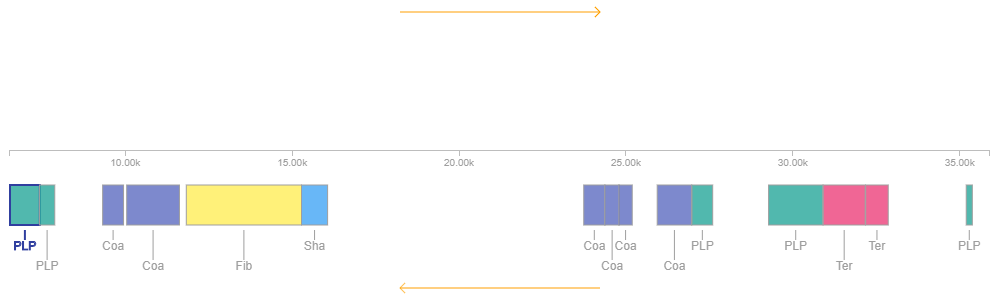
\includegraphics[width=1\linewidth]{img/circular_genome_node8_annotated}
	\caption{Node 8 of \textbf{FAM19191} assembly showing annotated locus. The highlited first one represents our muramidase.}
	\label{fig:circulargenomenode8annotated}
\end{figure}


\end{document}